\documentclass[11pt]{article}

\usepackage[margin=1in]{geometry}
\usepackage{booktabs}
\usepackage{array}
\usepackage{float}
\usepackage{amsmath}
\usepackage{hyperref}
\usepackage{enumitem}
\usepackage{graphicx}

\title{Task 1: Data Quality and Initial Exploratory Assessment\\
	Marketing Campaign Performance Analysis}
\author{}
\date{\today}

\begin{document}
	
	\maketitle
	
	\section{Introduction}
	
	Prior to conducting business intelligence analysis, the advertising campaign dataset was evaluated to ensure its quality, reliability, and suitability for analysis. The objective of this assessment is to identify potential data quality issues, validate the performance metrics used throughout the project, examine unusual observations, and establish a set of baseline metrics that will guide subsequent business analysis.
	
	The dataset contains daily advertising campaign performance across multiple platforms, regions, target audiences, product categories, and creative types during the first quarter of 2024.
	
	\section{Data Quality Assessment}
	
	\subsection{Data Completeness}
	
	The dataset was examined for missing values to determine whether incomplete observations could affect subsequent analyses.
	
	\begin{itemize}
		
		\item \textbf{Revenue}
		
		A sample of these datapoints are shown in \textit{Fig. \ref{fig:missing_values}}. It can be seen that twenty observations (approximately 0.6\% of the dataset) contained missing revenue values.
		\begin{figure}[h]
			\centering
			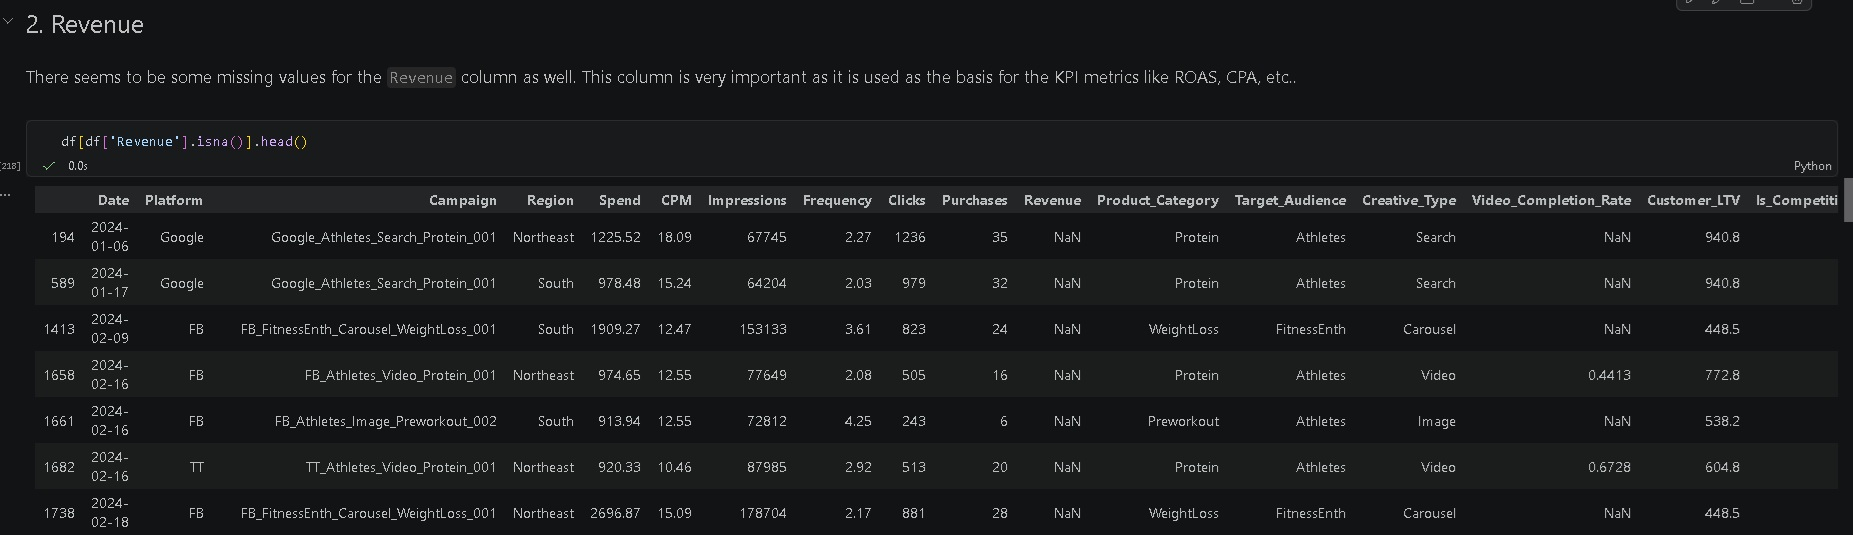
\includegraphics[width=1\textwidth]{images/revenue_missing_values.jpg}
			\caption{Sample datapoints with missing revenues.}
			\label{fig:missing_values}
		\end{figure}



		
		Because these represented a very small proportion of the data and no systematic pattern of missingness was identified, the corresponding observations were removed as shown in\textit{ Fig. \ref{fig:drop_missing_values}} prior to analysis.
	\begin{figure}[h]
		\centering
		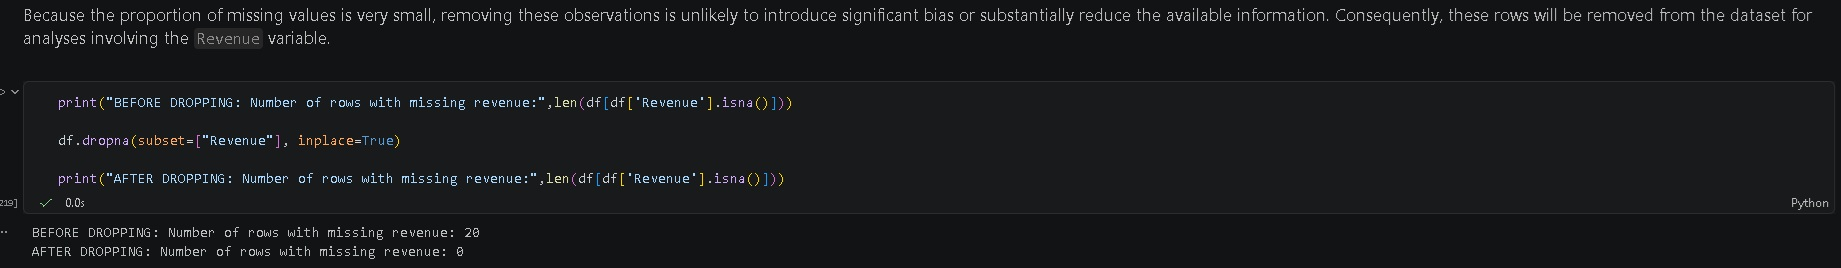
\includegraphics[width=1\textwidth]{images/drop_missing_revenue.jpg}
		\caption{Dropped datapoints with missing revenues.}
		\label{fig:drop_missing_values}
	\end{figure}
			
		
		\item \textbf{Video Completion Rate}
		
		A large number of missing values were initially observed in the \textit{Video Completion Rate} variable. Around 62\% of the total dataset! 
		
	\begin{figure}[h]
		\centering
		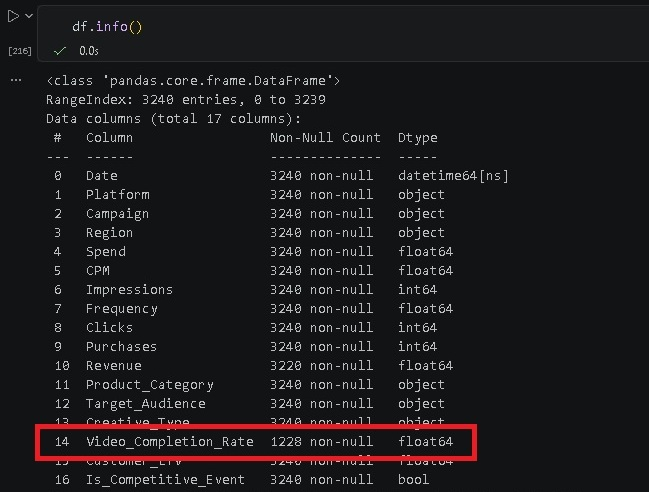
\includegraphics[width=0.45\textwidth]{images/video_completion_missing.jpg}
		\caption{Sample datapoints with missing video\_completion\_rate column}
		\label{fig:video_completion_missing}
	\end{figure}
		
		
		
		
		Further investigation revealed that this metric is only applicable to \textbf{campaigns using video advertisements}. After restricting the dataframe to video creatives, \textbf{only 212 missing observations remained} as shown in \textit{Fig. \ref{fig:filtered_video_completion_missing}}. 
		
	\begin{figure}[h]
		\centering
		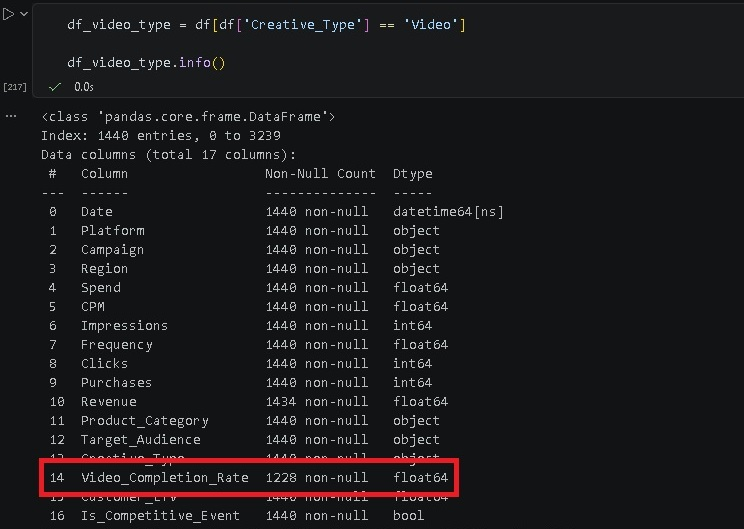
\includegraphics[width=0.45\textwidth]{images/filtered_video_completion_missing.jpg}
		\caption{DataFrame filtered to video creative types}
		\label{fig:filtered_video_completion_missing}
	\end{figure}	
		

		Consequently, these missing values were treated as \textbf{structurally missing} rather than data quality issues, and analyses involving this variable will use only the relevant subset of campaigns.
		
	\end{itemize}
	
	\subsection{Duplicate Records}
	
	The dataset was examined for duplicate observations.
	
	\begin{figure}[h]
		\centering
		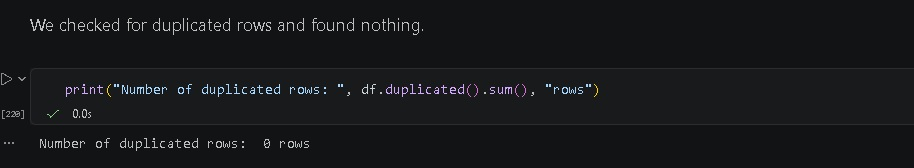
\includegraphics[width=0.8\textwidth]{images/duplicate_records.jpg}
		\caption{Checking for duplicate records}
		\label{fig:duplicate_records}
	\end{figure}
	
	
	No duplicate records were identified as shown in \textit{Fig. \ref{fig:duplicate_records}}.
	
	\subsection{Logical Consistency Checks}
	
	Several validation checks were performed to identify logically inconsistent observations.
	
	\subsubsection{0 Clicks with non-zero purchase}
	
	I noticed that there were rows with 0 clicks but has non-zero Purchases, which I thought was weird at first. How are they able to purchase without clicking the ad. 
	
	Apparently, this happens in real world scenarios and they are called \textbf{view-through conversions}. People see the ad, they don't click it then later that evening, they remembered the brand and typed the website into google and bought the product.
	
	\begin{figure}[h]
		\centering
		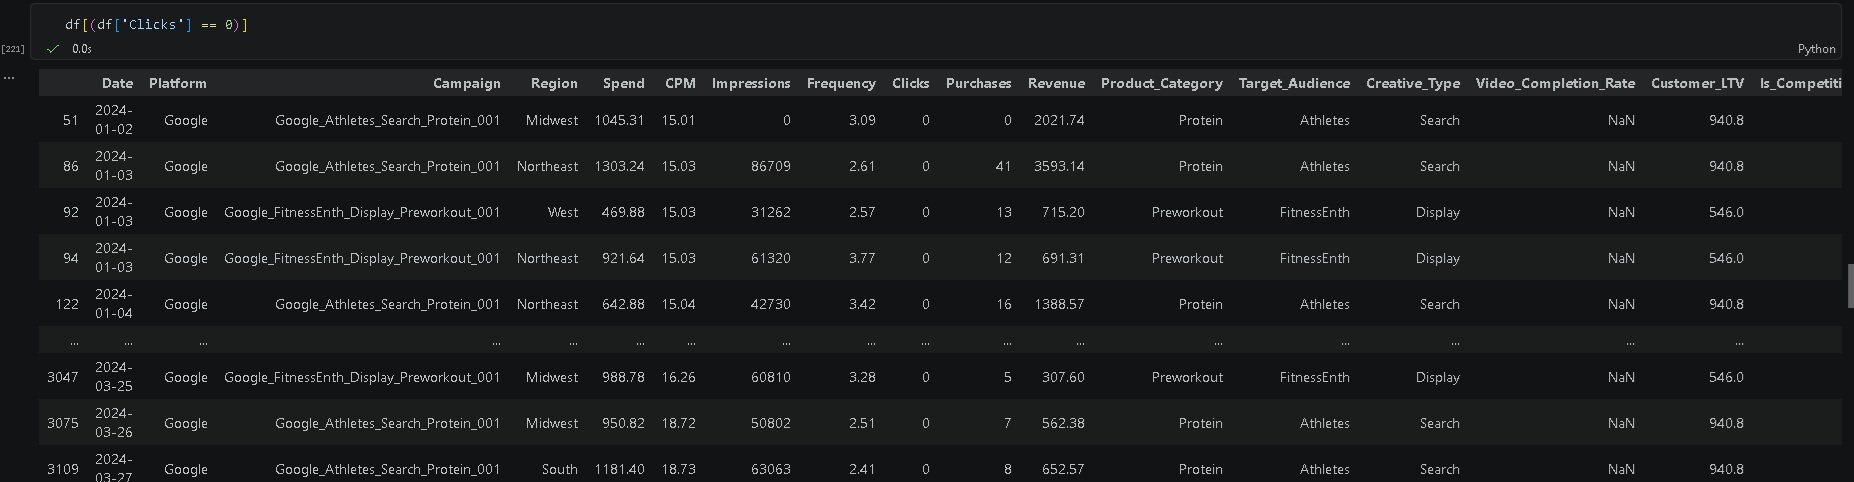
\includegraphics[width=0.8\textwidth]{images/0clicks_non0purchase.jpg}
		\caption{Sample datapoints with 0 clicks but non-zero purchase}
		\label{fig:0clicks_non0purchase}
	\end{figure}
	
	
	But, at this point, I was wondering how they know which ad actually influenced the purchased without click or what if the buyer interacted with multiple ads before purchasing(cross-channel conversions). Apparently, this is related to \textbf{attribution}, and there are multiple attribution models like \textbf{last\_click attribution}, \textbf{first-click attribution}, \textbf{linear\_attribution}, etc.. which is not part of this data cleaning process. 
	
	So, for now, I'll just assume that this dataset was collected using a certain attribution model and leave it at that. This justifies the 0 clicks with non-zero purchase.
	
	\subsubsection{0 Impressions with non-zero Cost-Per-Mile(CPM)}
	
	Cost Per Mille (CPM) measures the advertising cost required to generate 1,000 impressions and is commonly used to evaluate the cost efficiency of awareness campaigns.
	
	\begin{equation}
		\text{CPM} = \frac{\text{Spend}}{\text{Impressions}} \times 1000
	\end{equation}
	
	Because impressions appear in the denominator, CPM is undefined when the number of impressions is zero.
	
	During the data quality assessment, 47 observations (approximately 1.45\% of the dataset) were identified with \texttt{Impressions = 0} but non-zero CPM values. 
	

	Furthermore, all of these observations originated from the Midwest region as shown in \textit{Fig. \ref{fig:0impression}}, suggesting a systematic reporting inconsistency rather than isolated data entry errors.
	
	\begin{figure}[h]
		\centering
		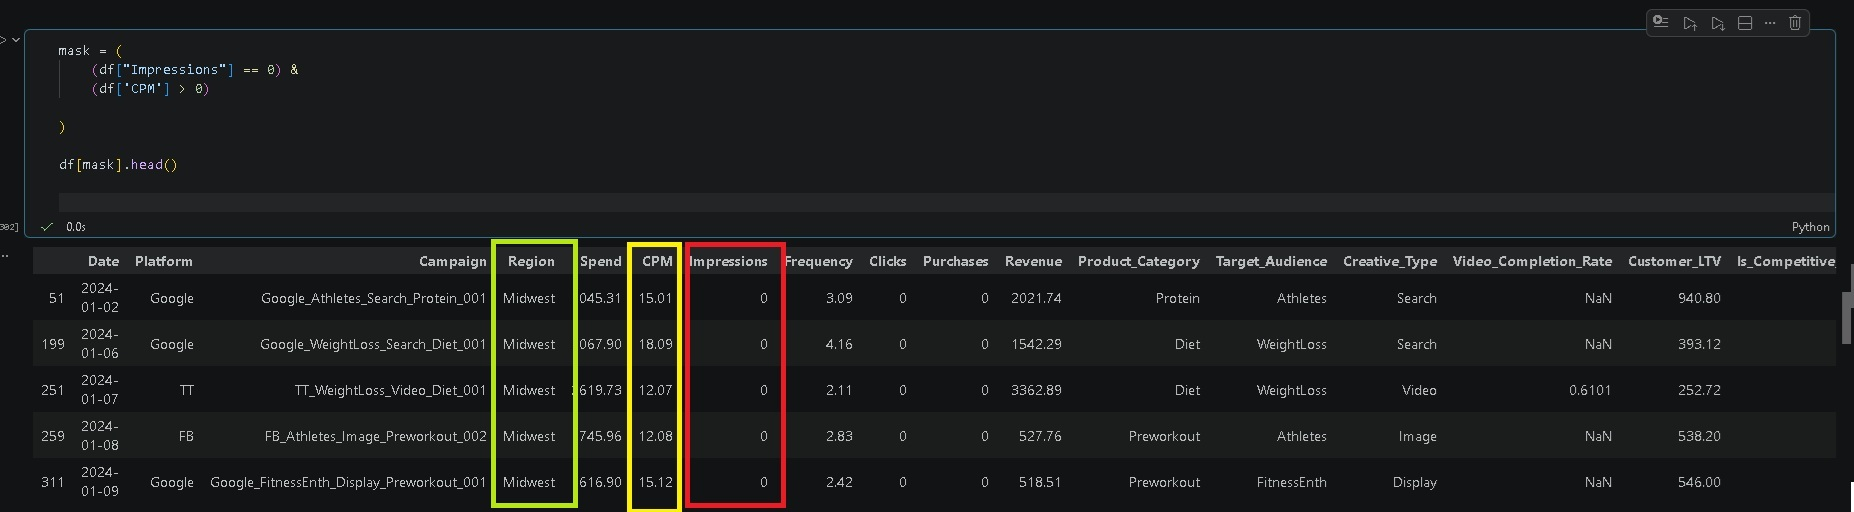
\includegraphics[width=0.8\textwidth]{images/0impressions.jpg}
		\caption{Sample rows that has 0 impressions with non-zero CPM}
		\label{fig:0impression}
	\end{figure}
	
	
	Since these observations violate the definition of CPM and could affect the calculation of other performance metrics, such as CTR and CVR, they were removed from the dataset prior to analysis.
	
	\begin{figure}[h]
		\centering
		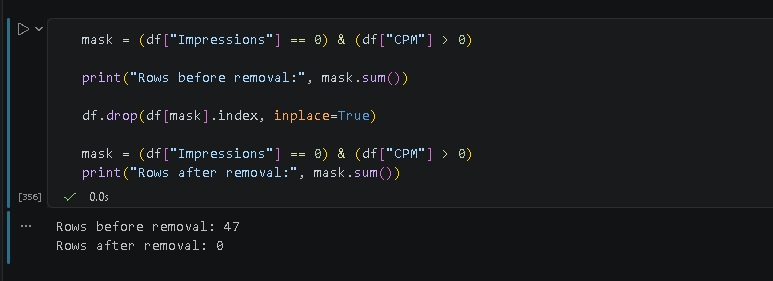
\includegraphics[width=0.8\textwidth]{images/0impressionscount.jpg}
		\caption{Dropped Rows that has 0 impressions with non-zero CPM}
		\label{fig:0impression_count}
	\end{figure}

	
	\subsection{Data Cleaning Summary}
	
	The data cleaning process consisted of:
	
	\begin{itemize}
		
		\item Removing observations with missing revenue.
		
		\item Removing logically inconsistent CPM observations.
		
		\item Retaining structurally missing Video Completion Rate values.
		
		\item Retaining valid view-through conversions.
		
		\item Verifying duplicate observations and variable data types.
		
	\end{itemize}
	
	Overall, the dataset was determined to be sufficiently complete and reliable for subsequent analysis.
	
	\section{Performance Metric Validation}
	
	To evaluate campaign effectiveness, four standard digital marketing performance metrics were calculated.
	
	\begin{table}[H]
		\centering
		\begin{tabular}{ll}
			\toprule
			Metric & Formula\\
			\midrule
			CTR & Clicks / Impressions\\
			CPC & Spend / Clicks\\
			CVR & Purchases / Clicks\\
			ROAS & Revenue / Spend\\
			\bottomrule
		\end{tabular}
		\caption{Calculated performance metrics.}
	\end{table}
	
	These metrics provide standardized measures of audience engagement, advertising efficiency, conversion effectiveness, and financial return.
	
	\subsection*{Click-Through Rate (CTR)}
	
	\textbf{Observation}
	
	CTR varies noticeably across campaigns, indicating substantial differences in audience engagement.
	
	\textbf{Why it Matters}
	
	Low CTR may indicate ineffective creative design, messaging, or audience targeting and warrants further investigation.
	
	\subsection*{Cost Per Click (CPC)}
	
	\textbf{Observation}
	
	CPC differs considerably between campaigns, suggesting variation in the cost required to generate user engagement.
	
	\textbf{Why it Matters}
	
	Campaigns with unusually high CPC may reduce advertising efficiency, particularly if higher acquisition costs do not translate into increased conversions or revenue.
	
	\subsection*{Conversion Rate (CVR)}
	
	\textbf{Observation}
	
	Several campaigns exhibit relatively high CTR but comparatively low CVR.
	
	\textbf{Why it Matters}
	
	This suggests that while advertisements successfully attract user attention, they are less effective at converting interest into purchases. Further investigation of post-click experiences is therefore warranted.
	
	\subsection*{Return on Advertising Spend (ROAS)}
	
	\textbf{Observation}
	
	ROAS varies substantially across campaign observations. Several high-spending campaigns generated comparatively low ROAS.
	
	\textbf{Why it Matters}
	
	Improving ROAS is the primary business objective. Consequently, identifying the factors associated with low ROAS will be a major focus of the subsequent business analysis.
	
	\section{Initial Exploratory Assessment}
	
	\subsection{Outlier Assessment}
	
	Numerical variables were examined using the Interquartile Range (IQR) method.
	
	Several variables, including advertising spend, impressions, revenue, and customer lifetime value, contained extreme observations. Manual inspection found no evidence that these observations resulted from data entry errors or impossible values. Instead, they represented legitimate campaign outcomes occurring across multiple platforms, regions, and campaign types.
	
	Accordingly, the identified outliers were retained to preserve meaningful variation within the dataset.
	
	\subsection{Baseline Performance Metrics}
	
	Given the business objective of improving advertising efficiency while optimizing budget allocation, the following metrics were selected as the primary indicators of campaign performance.
	
	\begin{table}[H]
		\centering
		\begin{tabular}{lp{10cm}}
			\toprule
			Metric & Business Relevance\\
			\midrule
			Spend & Measures advertising investment and budget allocation.\\
			
			Revenue & Measures the financial return generated by advertising activities.\\
			
			ROAS & Primary indicator of advertising efficiency and overall campaign profitability.\\
			
			CTR & Measures audience engagement with advertisements.\\
			
			CPC & Measures the cost required to acquire user engagement.\\
			
			CVR & Measures the effectiveness of converting engaged users into customers.\\
			
			\bottomrule
		\end{tabular}
		\caption{Baseline performance metrics used throughout the analysis.}
	\end{table}
	
	Together, these metrics evaluate campaign performance across the marketing funnel, from advertising investment and user engagement to customer conversion and financial return.
	
	\subsection{Preliminary Insights}
	
	The initial assessment identified several observations that warrant further investigation.
	
	\begin{itemize}
		
		\item Campaign performance varies considerably across the dataset.
		
		\item High advertising expenditure does not consistently produce higher ROAS.
		
		\item Some campaigns successfully attract user engagement but convert relatively few purchases, as indicated by high CTR and comparatively low CVR.
		
		\item Other campaigns demonstrate both high engagement and strong conversion performance, suggesting opportunities to identify characteristics associated with successful campaigns.
		
		\item These initial findings motivate further analysis by advertising platform, creative type, product category, target audience, geographic region, and competitive events.
		
	\end{itemize}
	
	\section{Key Assumptions}
	
	The following assumptions were adopted throughout the analysis.
	
	\begin{enumerate}
		
		\item Missing Video Completion Rate values are structural because the metric is only applicable to video advertisements.
		
		\item View-through conversions represent legitimate customer behavior and are therefore retained.
		
		\item Campaign performance comparisons should be based on aggregated campaign metrics rather than averages of daily ratios.
		
		\item Extreme observations represent genuine campaign performance unless evidence indicates otherwise.
		
	\end{enumerate}
	
	\section{Conclusion}
	
	The data quality assessment indicates that the advertising campaign dataset is suitable for subsequent business analysis following a limited number of cleaning operations. Missing values and logical inconsistencies were addressed appropriately, while valid observations representing legitimate campaign behavior were retained.
	
	The calculated performance metrics establish a consistent framework for evaluating advertising effectiveness. The preliminary assessment also highlights meaningful variation in campaign performance, particularly regarding engagement, conversion, and advertising return. These findings provide the foundation for the next phase of the project, where business intelligence techniques will be used to investigate campaign performance across multiple business dimensions and develop data-driven recommendations.
	
\end{document}